%# -*- coding: utf-8-unix -*-
%%==================================================
%% chapter02.tex for SJTU Master Thesis
%% based on CASthesis
%% modified by wei.jianwen@gmail.com
%% Encoding: UTF-8
%%==================================================

\chapter{过程控制系统的错误序列注入攻击}
\label{chap:FSIattack}

\section{引言}
\label{sec:intro}

过程控制系统作为国家关键基础设施的基本组成部分已经广泛应用于工业和物联网系统中。正因为它们在现代工业社会中的关键作用,使得它们成为怀有恶意目的的攻击者的感染和侵袭的目标。传统的安全保护主要是通过多层网络防火墙和成熟的的病毒防御软件阻止网络攻击入侵工业网络。然而考虑到网络和复杂的硬件系统实施,这些方法不能完全保护网络和硬件平台免受不断变异的威胁侵入,例如Stuxnet病毒侵入人机界面(HMI)服务器并上传恶意代码到可编程逻辑控制器PLC使其损坏制造核原料的离心机。考虑到HMI服务器通常安放在在受良好保护的工业控制网络中,所以对其实施攻击是非常困难的。
本章我们提出的错误序列注入(FSI)攻击,可以通过感染和篡改PLC的输入信号迫使其执行误操作和破坏控制系统的关键设备。因为PLC的输入仅仅来自假设被FSI攻击注入的远程传感器,所以在不需要渗透到防御坚固的控制网络并执行恶意代码上传的情况下便可以对系统实施有目的性攻击。值得注意的是我们构造的攻击可以避开现有的系统故障检测机制,并利用其容错率漏洞来构造基于离散时间模型的FSI攻击。

\section{攻击模型概述}
\label{sec:formulation}

考虑到图1描述的威胁模型,攻击者只需要侵入并控制遍布在远程的信号采集传感器。从过去的假数据注入攻击研究[5],[9],[19],[20],[30]中我们知道大部分工业控制系统包括电力系统的远程传感器如相量测量单元在实践中受到的保护较少并且分布在全国各地,因此与控制网络内的服务器相比更容易访问和侵入。我们假设攻击者知道高级基础设施配置,即连接到PLC传感器和执行器的输入输出的变量映射关系,这样攻击者不必渗透到控制网络中FSI攻击仍然可以成功。即使HMI服务器没有泄密而且攻击者也没有获得在PLC设备上上传恶意控制器程序的权限,我们构造的错误序列攻击只需要注入并控制向PLC发送测量信号的传感器便可以对控制系统造成不可逆的破坏。

\begin{figure}[!htb]
  \centering
  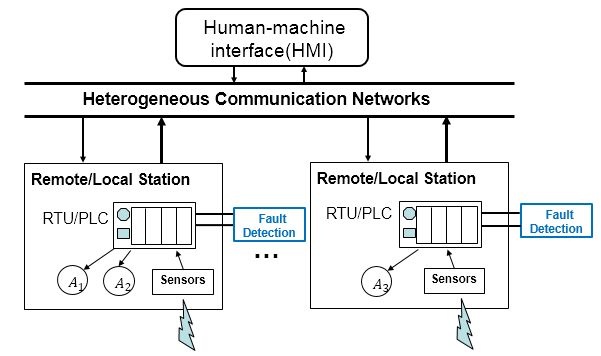
\includegraphics[scale=0.29]{threatModel1.png}
  \caption{FSI攻击威胁模型}
  \label{fig1}
\end{figure}

然而困难是如何在现有控制系统中部署的成熟故障检测的情况下构建攻击使PLC执行误动作。FSI攻击的主要任务之一是分析并且绕开故障检测机制。通常来看用辨识精度不高的系统模型来检测随机性的故障能够得到很高的准确度,我们通过这一特性反向构造错误序列并且注入到受控制的远程传感器则可以达到使故障检测失效的目的。图\ref {fig2}显示了攻击是如何构造的。我们假设对手可以访问在PLC控制器和物理设备之间交换的信号或堆栈数据。然后利用输入和输出向量数据库,我们辨识出与故障检测的建模方法类似的无故障的离散事件模型。最后,我们搜索所有的不可被故障机制检测的虚假序列的集合,并且获得适当长度的恶意序列对受控制的传感器采集的输入信号进行篡改。

\begin{figure}[!htb]
  \centering
  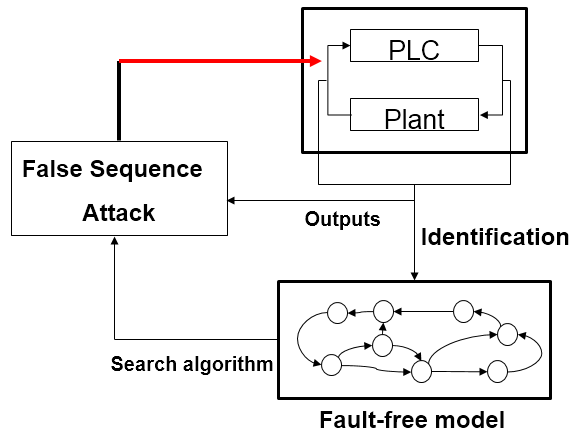
\includegraphics[scale=0.3]{ASC2.png}
  \caption{FSI攻击构造示意图}
  \label{fig2}
\end{figure}

\section{系统建模和攻击构造}
\label{sec:model}


\section{实验仿真}
\label{sec:simulation}

\section{本章小结}
\label{sec:insertimage}

